\documentclass[11pt,a4paper]{article}

\usepackage[applemac]{inputenc} %Careful with that Captain Ol.
\usepackage{latexsym}
\usepackage{graphicx}
\usepackage[francais]{babel}
\usepackage{amsmath,amssymb}
\usepackage{pstricks,pst-plot}
\usepackage{calc}
\usepackage{multicol}
\usepackage{fancyhdr}
\usepackage{lastpage}
\usepackage[T1]{fontenc}
\usepackage{stmaryrd}
\usepackage{float}
\pagestyle{plain}



\begin{document}

\section{Learning in discrete graphical models}

Let $(x_1, z_1), \ldots, (x_N, z_N)$ be an i.i.d. sample of observations. We will denote $n_m$ the number of $z_i$s which are equal to $m$ ($m \in \llbracket 1, M \rrbracket$). We have $\sum\limits_{m=1}^{M} n_m = N$.
%\\We compute the likelihood for Z: $\mathcal{L} = \mathop{\Pi}\limits_{i=1}^N p(Z = z_i) = \mathop{\Pi}\limits_{m=1}^M \pi_m^{n_m}$.
%\\Thus the log likelihood is equal to $\ell = \mathcal{L} = \sum\limits_{m=1}^M n_m \mathrm{log} \pi_m$.
%
\\In a similar fashion, for $k \in \llbracket 1, K \rrbracket$ and $\llbracket 1, M \rrbracket$ respectively, we denote $p_{mk}$ the number of $x_i$s equal to $k$, and whose label is equal to $m$. 
\\For a fixed $m$; we have $\sum\limits_{k=1}^{K}  p_{mk} = n_m$
\\We compute the likelihood for $\theta$ and $\pi$ : 
$$\begin{aligned} \mathcal{L} &= \mathop{\Pi}\limits_{i=1}^N p(X = x_i, Z = z_i) \\
 &= \mathop{\Pi}\limits_{i=1}^N p(X=x_i | Z= z_i) p(Z=z_i)\\
 & = \mathop{\Pi}\limits_{m=1}^M  \mathop{\Pi}\limits_{k=1}^K (\theta_{m k} \pi_m)^{p_{mk}} \\
  \end{aligned}$$
  %
Hence the log likelihood is equal to
 %
 $$\begin{aligned} \ell & = \sum\limits_{m=1}^M  \sum\limits_{k=1}^K p_{mk} \mathrm{log}(\theta_{m k} \pi_m) \\
 &= \sum\limits_{m=1}^M  \sum\limits_{k=1}^K p_{mk} \mathrm{log}(\theta_{m k})  +  \sum\limits_{m=1}^M  \sum\limits_{k=1}^K p_{mk} \mathrm{log}(\pi_m) \\
&= \sum\limits_{m=1}^M  \sum\limits_{k=1}^K p_{mk} \mathrm{log}(\theta_{m k})  +  \sum\limits_{m=1}^M  n_m \mathrm{log}(\pi_m) 
 \end{aligned}$$
 \\We are going to maximize this quantity with respect to $\pi$, and then with respect to $\Theta_1 = (\theta_{11}, \ldots, \theta_{M1})$, then $\Theta_2 = (\theta_{12}, \ldots, \theta_{M2})$, etc.
 \\[5mm]First we want to maximize the llh wrt $\pi$ under the following constraint : $\sum\limits_{m=1}^{M} \pi_m = 1$. Using a Lagrange multiplier method, we have that for $\pi$ maximizing the llh, there exists $\lambda$ such that 
 $$\forall m \in \llbracket 1, M \rrbracket, \frac{n_m}{\pi_m} = \lambda \times 1$$
\\that is 
$$\forall m \in \llbracket 1, M \rrbracket, n_m = \lambda \pi_m$$
\\if we sum these $m$ equalities, since $\sum\limits_{m=1}^{M} n_m = N$ and $\sum\limits_{m=1}^{M} \pi_m = 1$, we get $\lambda = N$.
So the likelihood is maximal wrt $\pi$ iff $$\forall m \in \llbracket 1, M \rrbracket,  \pi_m = n_m/N$$
which is a very natural result : the estimator for $p(Y=m)$ is just the proportion of observations $z_i$ equal to $m$.
%
\\[5mm]Now for every $k$ we must maximize the llh wrt $\Theta_k = (\theta_{1k}, \ldots, \theta_{Mk})$ with the constraint that $ \sum\limits_{m=1}^{M}  \theta_{mk} = 1$
\\Again we use a Lagrange multiplier.
\\At a point of maximum log likelihood wrt $\Theta_k$, we must have:
%
$$\frac{p_{mk}}{ \theta_{mk}} = \lambda_k \times 1$$
\\Which is equivalent to $p_{mk} = \lambda_k \theta_{mk}$
\\Summing on $m$ we get $n_k = \lambda \times 1$
\\Hence $\theta_{mk} = \frac{p_{mk}}{n_k}$.

%
%
%
%
\section{Linear classification}
%
%
%
\subsection{Generative model (LDA)}
%
%
\hspace*{-6mm}(a) The likelihood of this model can be written : 
%
$$\mathcal{L} = \mathop{\Pi}\limits_{i=1}^N ((1-\pi) f_0(x_i) + \pi f_1(x_i))$$
%
\\where $\pi = P(Y = 1)$ and $f_i$ is the density of a Gaussian law of mean $\mu_i$ and covariance matrix $\Sigma$.
\\ $f_i(x) = {1 \over 2 \pi |\Sigma|^{1/2}} e^{(x-\mu_i)^{T} \Sigma^{-1} (x-\mu_i) / 2}$
\\Then, the log likelihood is : $\ell =  \sum\limits_{i=1}^N n_k \mathrm{log} \pi_k$
\\As an estimator of $\pi$, we have in the same way as previously : $\pi = n/N$ 
\\And by derivating $\ell$ we obtain as estimators of $\mu_i$ and $\Sigma$ :
\\$\mu_i = \sum\limits_{k=1}^N x_{i,k}/n_i$ with $x_{i,k}$ the $x$s in the cluster i.
\\$\Sigma = \sum\limits_{i=0}^1 \sum\limits_{k \, \mathrm{st} \, y_k = i} (x_{i,k} - \mu_i) (x_{i,k} - \mu_i)^{T} / (N-2)$ %cours Gillou
%
%
\\[5mm](b) The form of the conditional distribution is :
\\$P(y=1|x) = {P(y=1) P(x|y=1) \over P(x)} = {1 \over 1+{\pi \over 1-\pi} f_0(x)/f_1(x)}$
\\If we take $\pi = 1/2$ and $w = \Sigma^{-1} (\mu_0 - \mu_1)$ and the constant
$b = (\mu_1^{T} \Sigma^{-1} \mu_1 + \mu_0^{T} \Sigma^{-1} \mu_0)/2$ we find the same result as for logistic regression.
%
%
\\[5mm] Here are the separators obtained on the 3 train datasets (black lines): 

\begin{figure}[H]
\centering
\noindent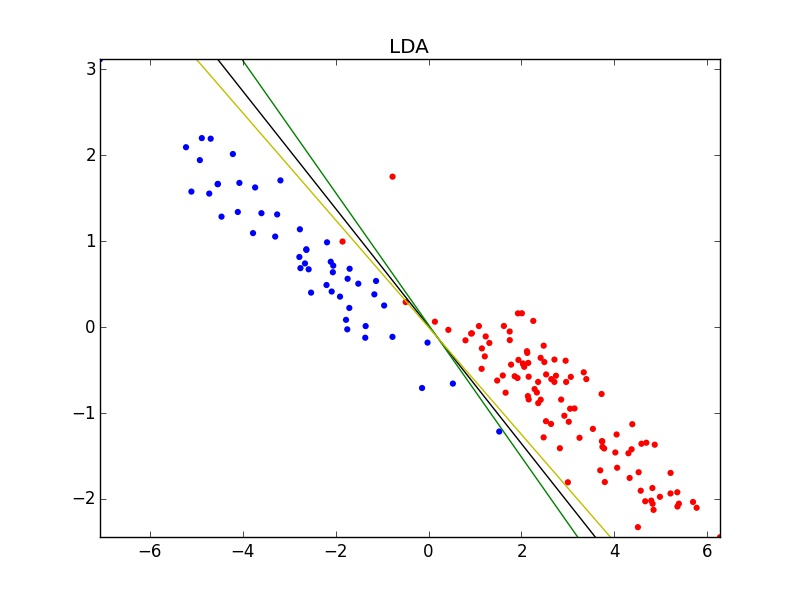
\includegraphics[scale=0.3]{images/LDA_A.jpeg}
\noindent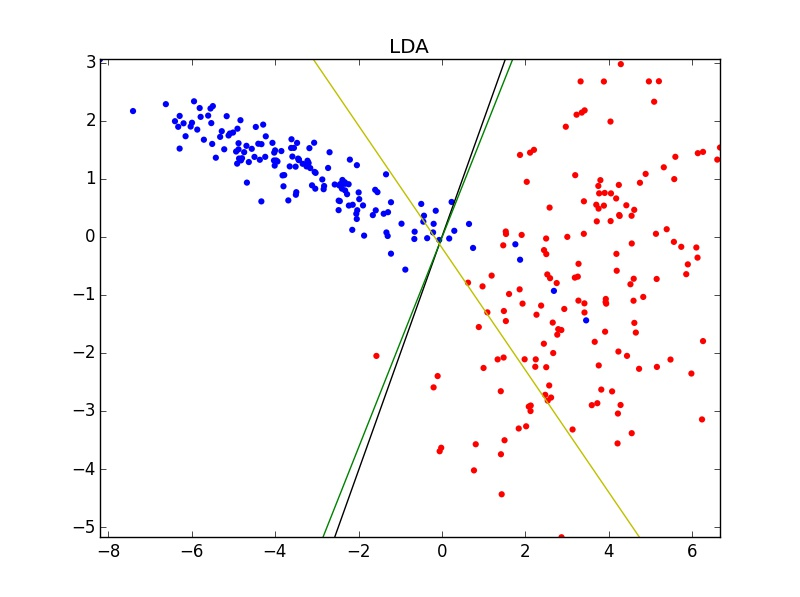
\includegraphics[scale=0.3]{images/LDA_B.jpeg}
\noindent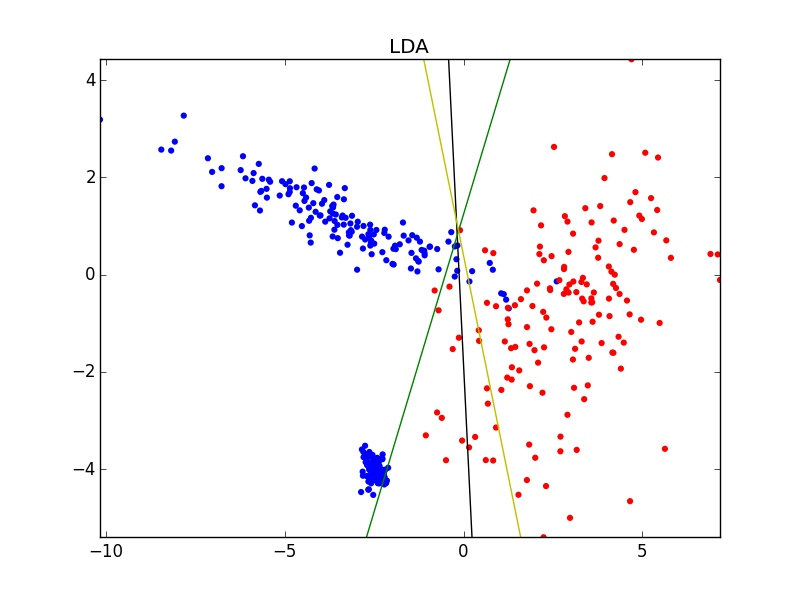
\includegraphics[scale=0.3]{images/LDA_C.jpeg}
\caption{Top: dataset A; middle: dataset B; bottom: dataset C}
\end{figure}

\subsection{Logistic regression}

\hspace*{-6mm}(a) On dataset A, we obtained : $w_A = (-0.706, -0,029)$.
\\On dataset B : $w_B = (1.766, -1,096)$.
\\And on dataset C : $w_C = (4.408, -1.613)$
%
%
\\[5mm](b) Here are the separators obtained on the 3 train datasets : 

\begin{figure}[H]
\centering
\noindent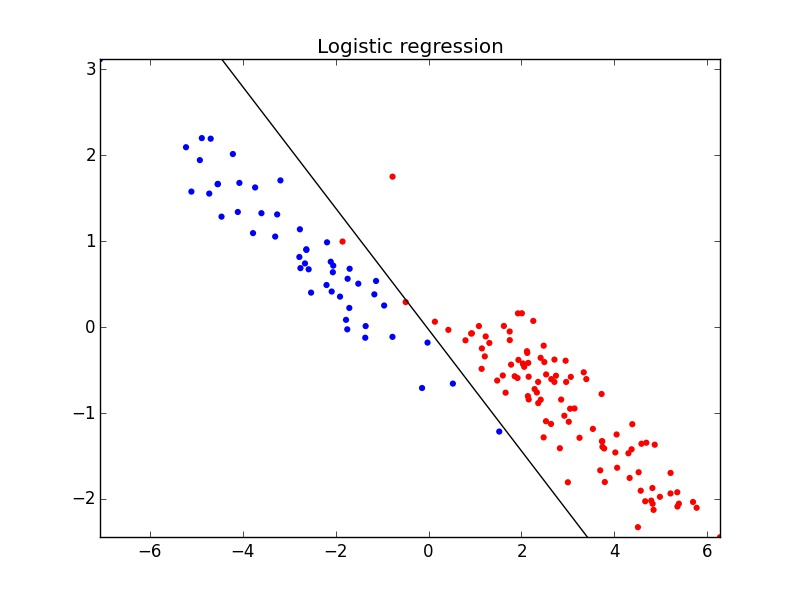
\includegraphics[scale=0.2]{images/logistic_A.jpeg}
\noindent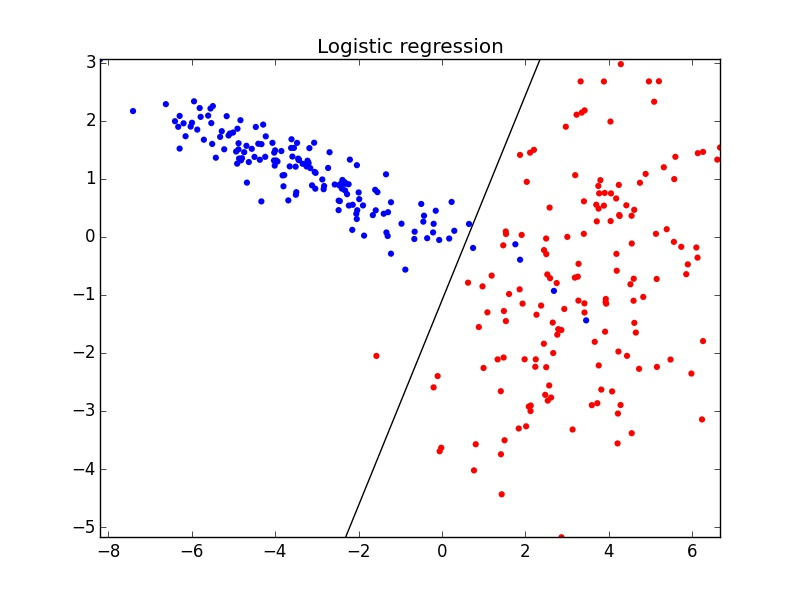
\includegraphics[scale=0.2]{images/logistic_B.jpeg}
\noindent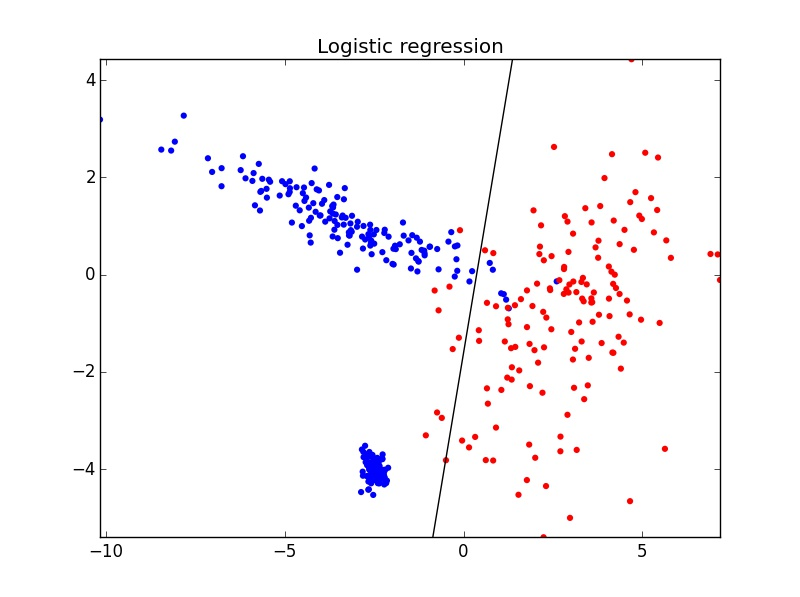
\includegraphics[scale=0.2]{images/logistic_C.jpeg}
\caption{Top-left: dataset A; top-right: dataset B; bottom: dataset C}
\end{figure}

\subsection{Linear regression}
%
\hspace*{-6mm}(a) On dataset A, we obtained : $w_A = (-0.709, -0,021)$.
\\On dataset B : $w_B = (2.013, -0.001)$.
\\And on dataset C : $w_C = (-7.511, 0.494)$
%
%
\\[5mm]Here are the separators obtained on the 3 train datasets : 

\begin{figure}[H]
\centering
\noindent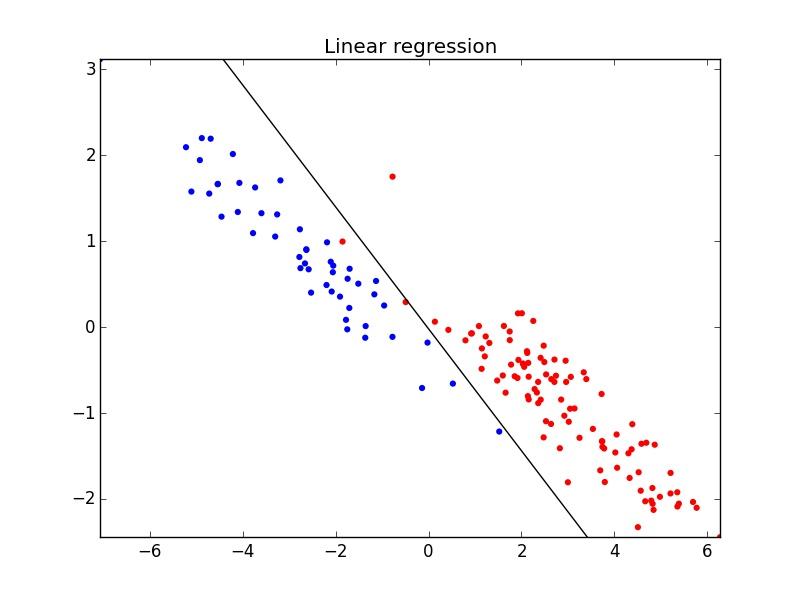
\includegraphics[scale=0.2]{images/linear_A.jpeg}
\noindent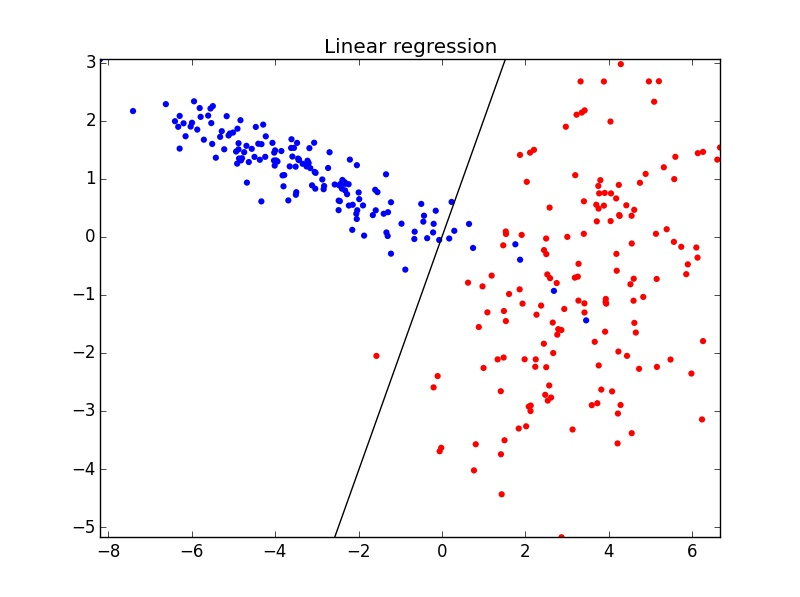
\includegraphics[scale=0.2]{images/linear_B.jpeg}
\noindent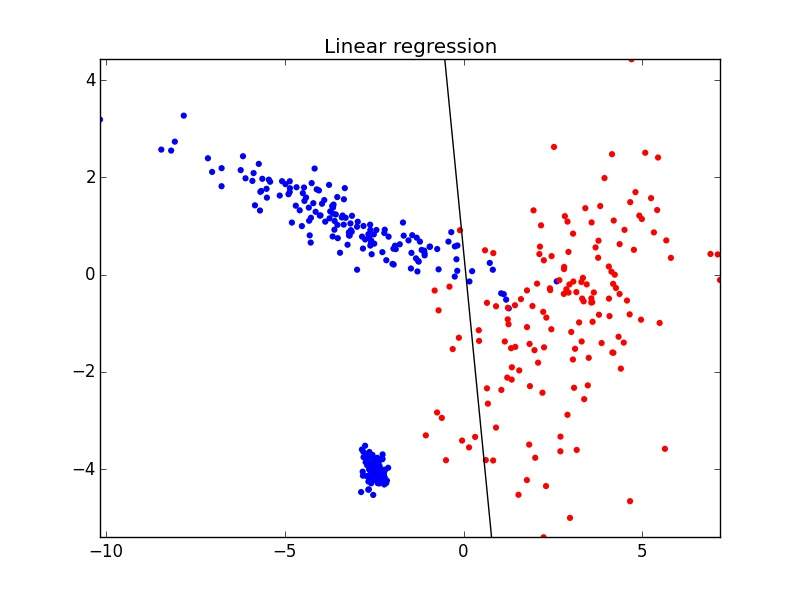
\includegraphics[scale=0.2]{images/linear_C.jpeg}
\caption{Top left: dataset A; top right: dataset B; bottom: dataset C}
\end{figure}

\subsection{QDA model}
%
\hspace*{-6mm}Here are the separators obtained on the 3 train datasets : 

\begin{figure}[H]
\centering
\noindent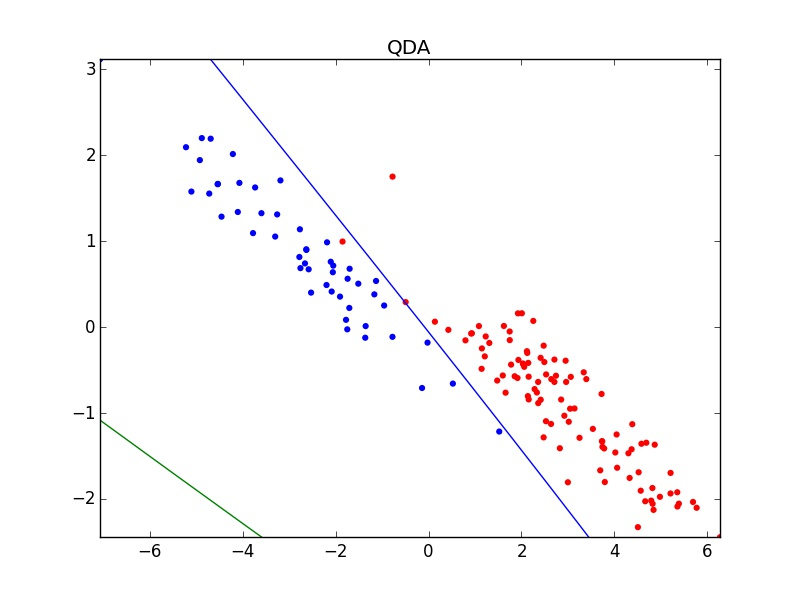
\includegraphics[scale=0.2]{images/qda_A.jpeg}
\noindent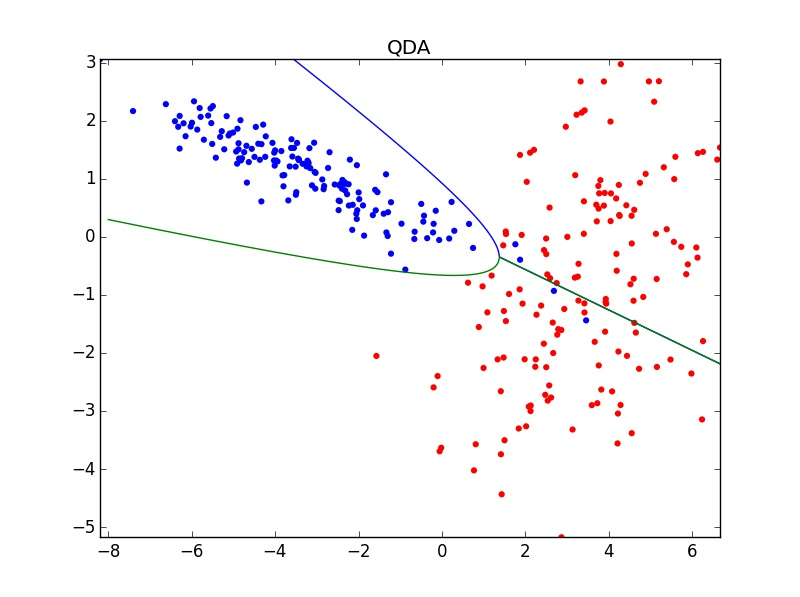
\includegraphics[scale=0.2]{images/qda_B.jpeg}
\noindent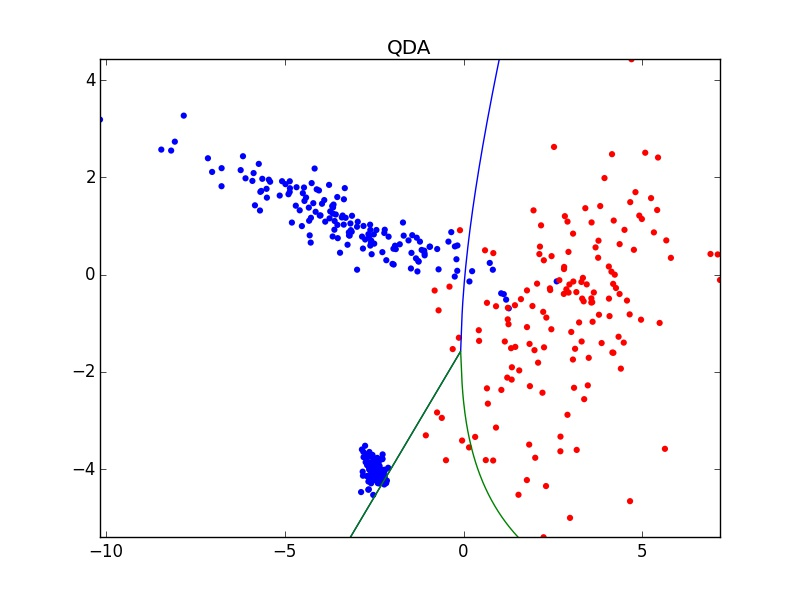
\includegraphics[scale=0.2]{images/qda_C.jpeg}
\caption{Top left: dataset A; top right: dataset B; bottom: dataset C}
\end{figure}

\subsection{Comparison}
%
\hspace*{-6mm}Here are the number of misclassification errors founded on train and test sets :



\end{document}